\section{Specification}
\label{sec:evaluationspecification}



\subsection{Evaluation Requirements}
\label{sec:evalrequirements}

% different message size, reduce loose couple being able to specify different types of messages
% invoke the endpoints with concurrent users and invoke endpoints concurrently
% be able to set the number of concurrent users and concurrent endpoints to invoke at the same time
% include multi-tenancy awareness in the benchmark for the different scenarios
% structured data as the output for analysis, for throughput and response time for the different messages requests for the different endpoints
% has to be done on top of the androitbenchmark, so that we can reuse and extend their benchmark
% system measurements of cpu and memory in structured data. also the measurement of the heap size (real memory consumtion) in the process
% monitoring of number of outgoing requests and incoming requests into the backend service, wireshark

In this student thesis we provide a performance analysis on the integration of the multi-tenant aware approaches in ServiceMix and measure the impact on the performance of the extended prototype. For this purpose, we need to fix which measurements we use for the evaluation. The driver should perform the following measurements: response time (measured in milliseconds) and throughput (measured in number of messages sent per second) respect to a backend service, and CPU and memory usage of the system hosting the instance of ServiceMix. The evaluation has to be done in different scenarios, each of them sending different messages number and sizes, for different multi-tenant and non multi-tenant aware endpoint configurations, as described in Table \ref{tab:evaluation} \cite{EvalESB}.

\begin{table}[htbp]
\centering
\begin{tabular}{llll}

	\toprule
	 Number of Endpoints 		& Messages Size	& ServiceMix Instances		& Multi-tenancy awareness 		\\
	 \midrule
	 
	 1 						& 0.5 / 1 KB 		& 1						& mt and non-mt									\\
	  						& 				& 2						& non-mt											\\
	 2 						& 0.5 / 1 KB 		& 1						& mt and non-mt									\\
	  						& 				& 2						& non-mt											\\
	 4 						& 0.5 / 1 KB 		& 1						& mt and non-mt									\\
	  						& 				& 2						& non-mt											\\
	 10 						& 0.5 / 1 KB 		& 1						& mt and non-mt									\\
	  						& 				& 2						& non-mt											\\														
	 
	\bottomrule
\end{tabular}
\caption[ServiceMix evaluation performance scenarios]{Specification of the different scenarios to be evaluated. In both multi-tenant and non multi-tenant aware evaluations, one user per endpoint / tenant is configured. \\ \term{Legend: mt (multi-tenant aware), non-mt (non multi-tenant aware)}}
	\label{tab:evaluation}
\end{table}

AndroitLogic has developed a performance analysis driver which fulfills most of the above requirements in different scenarios \cite{androit2012}. In our evaluation, we extend the Direct Proxy scenario from the AndroitLogic  \ac{ESB} Performance benchmark \cite{androit2012}. However, it doesn't achieve one of the main requirements of this student thesis: multi-tenant aware messaging and concurrent invocation between endpoints. Those two requirements should be included in an extended version of the primitive driver. Furthermore, the extension should be utilized with different \ac{ESB} solutions and must be user-friendly configurable for the different scenarios. The output of the driver measurements should be analyzed, therefore the output data must be in structured format. 

\subsection{Evaluation Overview}
\label{sec:evaluationoverview}

% main picture of the overview of the system for evaluating the esb and explain it with detais of the hardware setup of the vm
% describe a little bit the scenarios that were fixed
% 
In the Section \ref{sec:requirements} we have described the requirements that the evaluation should fulfill and the needed modifications in the utilized benchmark. As exposed in Figure \ref{fig:evaluationoverview}, the evaluation is conformed by three main independent systems. We must ensure, for analyzable purposes, that we approximate as much as possible to a Web service standard real scenario: service requester invokes a backend service and both request and response are routed through the network. In our evaluation we must utilize the \ac{ESB} as a mediator between the service requester and provider. In the first system (VM0), both service requestor and provider are deployed. The communication measurements are taken in two different components: throughput and response time in the AndroitLogic driver, while the number of incoming and outgoing requests, as well as the visualization of the messages, have to be monitored in an independent monitoring component. 

In the second and third systems (VM1 and VM2 respectively) one instance of ServiceMix is deployed for routing the messages between the AndroitLogic driver and the backend service. A monitor component must perform the counting of the incomming and outgoing requests to and from the \ac{ESB}, and a system monitor component should measure the \ac{ESB}'s resources consumption. The connection between the components in VM0 and VM2 is represented with a dashed line, because the VM2 is only use for non multi-tenant aware scenarios. Similarly, we have connected the components in VM0 with the components in VM1 with a continuos line, because this connection is used in both multi-tenant and non multi-tenant aware scenarios. 

The JBIMulti2 application is used for deployment of the \ac{SA}s which pack the endpoint configurations in the \ac{SU}s. However, we do not include the JBIMulti2 application in our overview because we do not evaluate the JBIMulti2 performance, but the multi-tenant and non multi-tenant ServiceMix independently from the JBIMulti2 application.

\begin{figure}[htb]
	\centering
		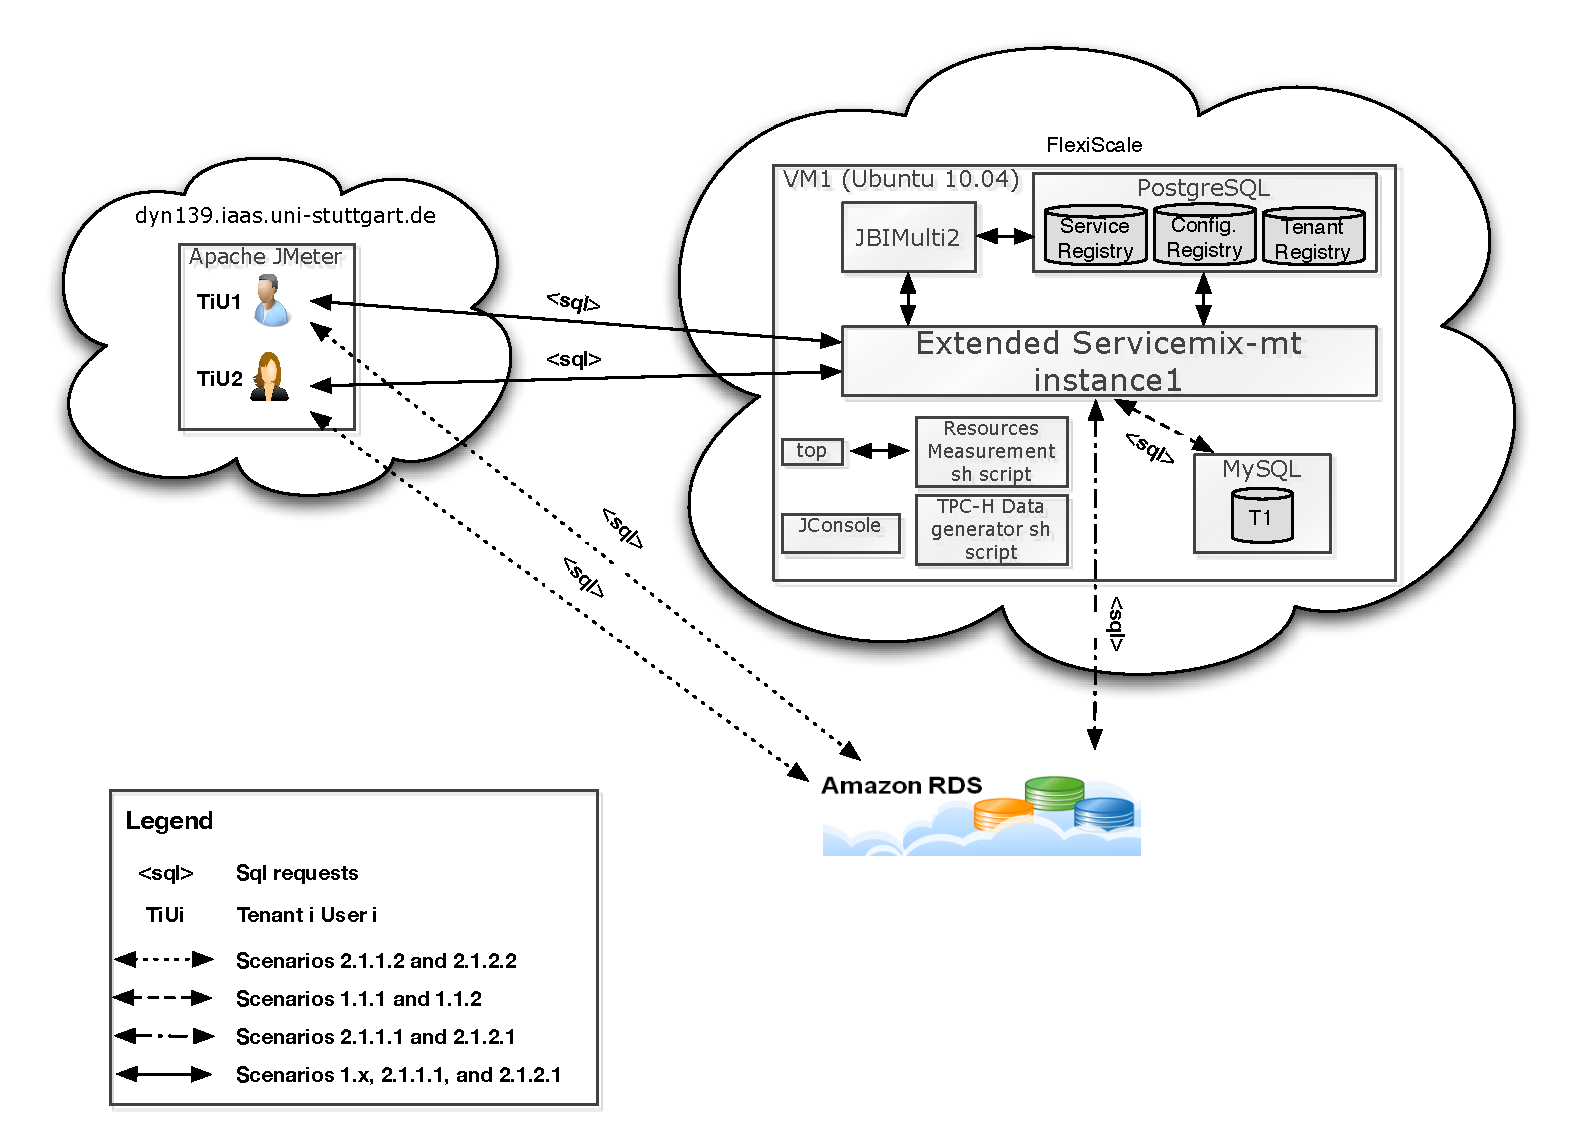
\includegraphics[width=0.7\textwidth, trim=0.0cm 0.0cm 0.0cm 0.0cm, clip]{./gfx/evaluationoverview.pdf}
	\caption[Performance Evaluation Components Overview]{Overview of the components used for the \ac{ESB} performance evaluation. \textbf{Note:} In the evaluation two different monitors are used. For communication the monitoring requires the counting and visualization of the incoming and outgoing requests. For system monitoring, the CPU and Memory usage should be measured.}
	\label{fig:evaluationoverview}
\end{figure}

\FloatBarrier

\FloatBarrier